\documentclass[a4paper,11pt]{report}
 
% Import des extensions
\usepackage[T1]{fontenc}
\usepackage[utf8]{inputenc}
\usepackage[francais]{babel}
\usepackage{graphicx}
\usepackage{color}
\usepackage{colortbl}
\usepackage{geometry}
\usepackage{hyperref}
\usepackage{fullpage}
\usepackage{eso-pic}
\geometry{hmargin=2.5cm,vmargin=3.5cm}


\newcommand{\blap}[1]{\vbox to 0pt{#1\vss}}
\newcommand\AtUpperLeftCorner[3]{%
\put(\LenToUnit{#1},\LenToUnit{\dimexpr\paperheight-#2}){\blap{#3}}%
}
\newcommand\AtTopCenterPage[2]{%
\put(\LenToUnit{.5\paperwidth},\LenToUnit{\dimexpr\paperheight-#1}){\blap{\hbox to 0pt{\hss#2\hss}}}%
}
\newcommand\AtUpperRightCorner[3]{%
\put(\LenToUnit{\dimexpr\paperwidth-#1},\LenToUnit{\dimexpr\paperheight-#2}){\blap{\llap{#3}}}%
}


\author{Dylan Bideau, Julien Turpin, Pierre Bogrand, Guillaume Vincenti}
\title{\huge{Nautilus - Rapport}}
\date{10 Avril 2018}

\begin{document}
\makeatletter
\begin{titlepage}

	\AddToShipoutPicture{
		\AtUpperLeftCorner{1.5cm}{1cm}{
\includegraphics[width=4cm]{Photos/ensea.png}}
	}
	\begin{center}
		\vspace*{10cm}
		\textsc{\@title}
		\vspace*{0.5cm}
		\hrule
		\vspace*{0.5cm}
		\large{\@author}
	\end{center}
	\vspace*{9.2cm}
	\begin{center}
		\large{\@date}
	\end{center}
\end{titlepage}
\ClearShipoutPicture

\renewcommand{\contentsname}{Sommaire}
\tableofcontents


\chapter{Introduction}

        Les fonds marins réunissent aujourd'hui de nombreux secteurs et enjeux, tant professionels que particuliers. On y retrouve entre autre l'exploration sous-marine, la surveillance et maintenance d'installations professionelles, ainsi que la cartographie des fonds marins. Tout ces domaines demandent le développement de solutions techniques plus rentables et pratiques qu'une intervention humaine. Notre projet propose ainsi un ROV (Remotely Operated Vehicle) polyvalent et simple d'utilisation à cet effet.

\chapter{Présentation du projet}
        
				Un ROV est un robot sous-marin contrôlé à distance et permettant une acquisition d'informations, visuelles ou à partir de capteurs. Notre projet de ROV filoguidé, Nautilus, sera transportable et pilotable à l'aide d'un ordinateur portable. Il permettra d'observer facilement des installations ou des fonds marins à l'aide de caméras. Disposant également de fonctions avancées, le Nautilus sera en mesure de recréer le fond marin d'une zone géographique déterminée par l'utilisateur à partir d'une batterie de photographies prises lors de la phase d'exploration. Les différentes fonctionnalités du Nautilus en font ainsi un outil polyvalent, permettant exploration, maintenance et cartographie des fonds.
				
				
\chapter{Cahier des charges}

        \section{Analyse Fonctionnelle}
						\subsection{Structure}
								Facilement transportable et peu emcombrant.\newline
								\textbf{Contraintes :}
								\begin{itemize}
										\item Poids : 2-3kg
										\item Dimension : 300*200*150mm
										\item Etanche de norme IP 68 \newline \newline
									\end{itemize}

						\subsection{Commandabilité}
								Commandé à distance par une liaison filaire.\newline
								\textbf{Contraintes :}
								\begin{itemize}
										\item Câble : 15m
										\item Carte intégrée dans le ROV
										\item FPV (First Person View)
										\item Piloté au clavier\newline \newline
								\end{itemize}

						\subsection{Milieu d'utilisation}
								Adapté aux contraintes imposées par son environnement. \newline
								\textbf{Contraintes :}
								\begin{itemize}
										\item Eau non salé (moins de 1 g de sels dissous par kilogramme d'eau)
										\item Eau translucide (transmittance de la lumière entre 75\% et 95\%)
										\item Lieu : Piscine, lac
										\item Ecoulement laminaire
										\item Courant marin inferieur à 2 noeuds
										\item Profondeur de 10m (résistant à 2 bars) \newline \newline
								\end{itemize}

						\subsection{Energie}
								Etre entièrement autonome. \newline
								\textbf{Contraintes :}
								\begin{itemize}
										\item Autonomie de 20 minutes
								\end{itemize}

						\subsection{Motorisation}
								Etre mobile une fois immergé. \newline
								\textbf{Contraintes :}
								\begin{itemize}
										\item Propulsion electrique
										\item Déplacement horizontal (Vitesse maximale de 1m/s)
										\item Déplacement vertical (Vitesse maximale de 0.5m/s)
										\item Direction droite/gauche à 360 degres   \newline \newline
								\end{itemize}

						\subsection{Acquisitions}
								Acquérir et transmettre l'information. \newline
								\textbf{Contraintes :}
								\begin{itemize}
										\item Acquisition et retransmission d'un signal vidéo
										\item Acquisition et stockage de photographies
										\item Mesure de la pression
										\item Mesure de la position relative avec signaux GPS
								\end{itemize}
								
\chapter{Motorisation et énergie}

				\section{Moteurs brushless et ESC} 
				
							Dans un premier temps, il a été question de la technologie des moteurs à utiliser. Après une étude des différentes solutions disponibles, nous avons finalement choisi des moteurs brushless (\href{http://www.conrad.fr/ce/fr/product/231891/Moteur-davion-lectrique-brushless-ROXXY-315079?ref=searchDetail}{Référence 1}). En effet, les moteurs brushless sont des machines synchrones auto-pilotées à aimants permanents et donc sans balais. \newline
			\begin{figure}[!h]
				\begin{center}
					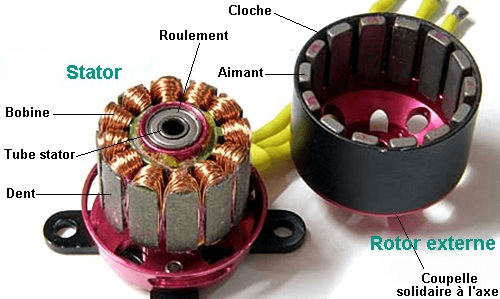
\includegraphics{Photos/moteur-brushless}
				\end{center}
			\end{figure}\newline
							Le principal avantage de ces moteurs est qu'ils peuvent être utilisés immergés dans l'eau sans aucun traitement particulier au préalable. En revanche, un système électronique de commande doit assurer la commutation du courant dans les enroulements statoriques : les ESC, ou Electronic Speed Controllers. Un ESC transforme un signal d'alimentation continu, dans notre cas issu d'une batterie, en un signal triphasé envoyé ensuite au moteur brushless. Pour contrôler la vitesse du moteur, on envoie à l'ESC un signal de commande, généralement créneau, et dont le rapport cyclique définit la vitesse du moteur. Les trois ESC commandés dans un premier temps (\href{https://www.robotshop.com/eu/fr/esc-multirotor-20a-m20a.html}{Référence 2})  
	
				\section{Calibration des ESC}
				
				\section{Alimentation et montage}
				(BEC)
				
				
\chapter{Références}

				\textbf{Motorisation et énergie :}
				\begin{itemize}
							\item \textbf{\href{http://www.conrad.fr/ce/fr/product/231891/Moteur-davion-lectrique-brushless-ROXXY-315079?ref=searchDetail}{Référence 1}} : Moteur d'avion électrique brushless ROXXY 315079 chez Conrad (x3)
							\item \textbf{\href{https://www.robotshop.com/eu/fr/esc-multirotor-20a-m20a.html}{Référence 2}} : ESC Suppo Multirotor 20A M20A chez RobotShop (x3)
										
				\end{itemize}

\end{document}
